\documentclass[tikz,border=10pt]{standalone}
\begin{document}
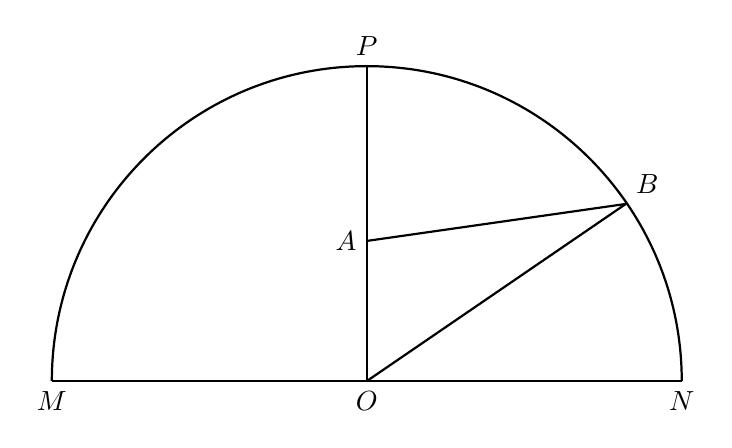
\begin{tikzpicture}[thick]
  \coordinate (M) at (-4,0);
  \coordinate (O) at (0,0);
  \coordinate (N) at (4,0);
  \coordinate (P) at (0,4);
  \coordinate (A) at (0,1.78);
  \coordinate (B) at (3.29,2.25);

  \draw (M) -- (N);
  \draw (O) -- (P);
  \draw (M) arc (180:0:4);
  \draw (A) -- (B);
  \draw (O) -- (B);

  \node[above] at (P) {$P$};
  \node[left] at (A) {$A$};
  \node[above right] at (B) {$B$};
  \node[below] at (O) {$O$};
  \node[below] at (M) {$M$};
  \node[below] at (N) {$N$};
\end{tikzpicture}
\end{document}
